\documentclass[11pt,oneside]{amsart}
\usepackage[margin=1in]{geometry}
\usepackage{amssymb,parskip,mathtools,microtype,tikz}
\usepackage[shortlabels]{enumitem}

\theoremstyle{definition}
\newtheorem{problem}{Problem}
\newtheorem{question}{Question}

\theoremstyle{plain}
\newtheorem{theorem}{Theorem}

\newcommand{\bC}{\mathbb{C}}
\newcommand{\bQ}{\mathbb{Q}}
\newcommand{\bR}{\mathbb{R}}
\newcommand{\bZ}{\mathbb{Z}}
\newcommand{\bE}{\mathbb{E}}
\newcommand{\BP}{{\mathbf{P}}}
\newcommand{\ba}{{\mathbf{a}}}
\newcommand{\bi}{{\mathbf{i}}}
\newcommand{\bj}{{\mathbf{j}}}
\newcommand{\bk}{{\mathbf{k}}}
\newcommand{\bn}{{\mathbf{n}}}
\newcommand{\br}{{\mathbf{r}}}
\newcommand{\bs}{{\mathbf{s}}}
\newcommand{\bu}{{\mathbf{u}}}
\newcommand{\bv}{{\mathbf{v}}}
\newcommand{\bw}{{\mathbf{w}}}
\newcommand{\eps}{\varepsilon}
\newcommand{\blank}{\underline{\hspace{1cm}}}
\newcommand{\longblank}{\underline{\hspace{2cm}}}

\DeclareMathOperator{\Var}{Var}
\let\Re\relax
\DeclareMathOperator{\Re}{Re}
\let\Im\relax
\DeclareMathOperator{\Im}{Im}
\DeclareMathOperator{\Res}{Res}
\DeclareMathOperator{\ord}{ord}
\DeclareMathOperator{\dir}{\mathbf{dir}}

\title{MATH2202 Spring 2024\\
Exam 2}
\author{Wednesday, April 10, 2024}

\begin{document}
\maketitle

Name: \underline{\hspace{6cm}}

This exam is open book. Calculators are not allowed. There are 50 points total in this exam. If you do not manage to solve a problem, show a strategy you tried and a reflection on why it did not work, for partial credit.

\vskip 2cm

Please answer the following questions.

\begin{question}
  I did the practice problems on the homework. (Circle one.)

  \hspace{1.5cm}Yes, all of them\hspace{1.5cm} Some of them\hspace{1.5cm} No
\end{question}

\begin{question}
  I did the midterm additional practice problems. (Circle one.)

  \hspace{1.5cm}Yes, all of them\hspace{1.5cm} Some of them\hspace{1.5cm} No\hspace{1.5cm}What's that?
\end{question}

\begin{question}
  I understood the homework solutions. (Circle one.)

  \hspace{1.5cm}Yes, all of them\hspace{1.5cm} Some of them\hspace{1.5cm} No
\end{question}

\begin{question}
  I can understand the textbook. (Circle one.)

  \hspace{1.5cm}Yes\hspace{1.5cm} Only the examples\hspace{1.5cm} No, but I tried\hspace{1.5cm}Didn't read
\end{question}

\begin{question}
  I come to class. (Circle one.)

  \hspace{1.5cm}Yes and I mainly listen\hspace{1.5cm}Yes and I take notes\hspace{1.5cm} No
\end{question}

\begin{question}
  I come to discussions. (Circle one.)

  \hspace{1.5cm}Yes\hspace{1.5cm} No
\end{question}

\begin{question}
  I studied using: (Circle all that apply.)

  \hspace{1.5cm}Homework solutions\hspace{0.05\textwidth} Practice problems\hspace{0.05\textwidth} Materials from previous years

  \hspace{1.5cm}Other (please specify): \underline{\hspace{8cm}}
\end{question}

\newpage

\begin{problem}\leavevmode
  \begin{enumerate}[(a)]
    \item (5 points) The point $(\rho,\theta,\phi)=(3,\pi/2,\pi/2)$ is given in spherical coordinates. What is it in rectangular coordinates?
    \vfill
    \item (5 points) Swap the order of integration of the following double integral, but do not evaluate.
    \[\int_1^4\int_{y}^{y^2}\frac 1y\,dx\,dy.\]
    Your answer should be of the form
    \[\int_{\boxed{?}}^{\boxed{?}}\int_{\boxed{?}}^{\boxed{?}}\boxed{?}\,dy\,dx+\int_{\boxed{?}}^{\boxed{?}}\int_{\boxed{?}}^{\boxed{?}}\boxed{?}\,dy\,dx.\]
    Drawing a picture is highly recommended.
    \vfill
    \vfill
    \vfill
  \end{enumerate}
\end{problem}

\newpage

\begin{problem}\leavevmode
  \begin{enumerate}[(a)]
    \item (5 points) Compute the triple integral
    \[\iiint_{\mathcal U}dV\]
    where $\mathcal U=\{(x,y,z)\mid 0\leq y\leq 2,2\leq z\leq 4, y\leq x\leq z\}$.
    \vfill
    \item (5 points) Write down (but do not solve) the Lagrange equations that would solve this problem: Find the point $(x,y,z)$ on the sphere of radius 6 centered at the origin closest to $(1,2,3)$.
    \vfill
  \end{enumerate}
\end{problem}

\newpage

\begin{problem}
  Let $f(x,y)=xe^y+3x$.
  \begin{enumerate}[(a)]
    \item (3 points) Calculate $\nabla f(5,0)$.
    \vfill
    \item (7 points) You're given that $\nabla f(3,0)=(4,3)$. Show that there is no unit vector $\bu$ such that $D_\bu f(3,0)=-6$.
    \vfill
    \vfill
    \vfill
  \end{enumerate}
\end{problem}

\newpage

\begin{problem}[10 points]
  The Archimiedean spiral $r=\theta$ is drawn below. Write down, but do not evaluate, an integral in polar coordinates that represents the shaded area. (Hint: Despite appearances, the arcs are not circular arcs.)
  \begin{center}
    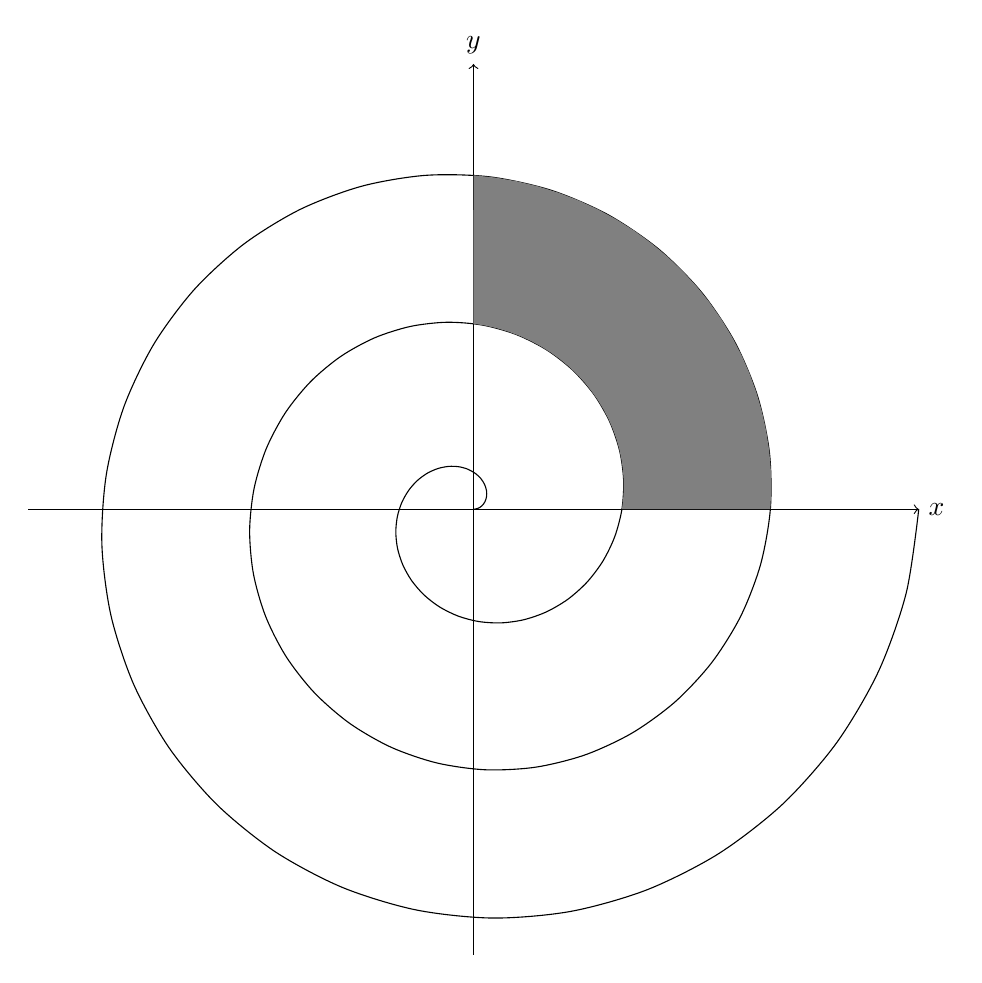
\begin{tikzpicture}[scale=0.3]
      \draw[->] (0,-6*pi) -- (0,6*pi) node[above] {$y$};
      \draw[->] (-6*pi,0) -- (6*pi,0) node[right] {$x$};

      \draw[domain=0:6*pi,smooth,variable=\t,samples=100] plot ({\t*cos(deg(\t))},{\t*sin(deg(\t))});
      \fill[gray] (2*pi,0) -- plot[domain=4*pi:4.5*pi, variable=\t] ({\t*cos(deg(\t))},{\t*sin(deg(\t))}) -- (0,4*pi) -- plot[domain=2.5*pi:2*pi, variable=\t] ({\t*cos(deg(\t))},{\t*sin(deg(\t))}) -- cycle;
    \end{tikzpicture}
  \end{center}
\end{problem}

\newpage

\begin{problem}[10 points]
  Recall that a (twice-differentiable) function $f(x,y)$ is \emph{harmonic} if it satisfies
  \[\frac{\partial^2 f}{\partial x^2}(x,y)+\frac{\partial^2 f}{\partial y^2}(x,y)=0\text{ for all }x,y.\]
  Suppose $f(x,y)$ is a harmonic function and that for every critical point $(x_0,y_0)$ of $f$, the discriminant $\mathcal D(f,(x_0,y_0))$ is nonzero. Prove that $f$ has no local minima or maxima.\footnote{The claim is still true without the discriminant condition but would be harder to prove.}

  Hint: Start with the following sentence: ``Suppose that $P=(x_0,y_0)$ is a critical point of $f$.'' You may use the space below for scratch work and/or thinking.
\end{problem}

\end{document}
